\documentclass[9pt,a4paper,]{extarticle}

\usepackage{f1000_styles}

\usepackage[pdfborder={0 0 0}]{hyperref}

\usepackage[numbers]{natbib}
\bibliographystyle{unsrtnat}


%% maxwidth is the original width if it is less than linewidth
%% otherwise use linewidth (to make sure the graphics do not exceed the margin)
\makeatletter
\def\maxwidth{ %
  \ifdim\Gin@nat@width>\linewidth
    \linewidth
  \else
    \Gin@nat@width
  \fi
}
\makeatother

\usepackage{color}
\usepackage{fancyvrb}
\newcommand{\VerbBar}{|}
\newcommand{\VERB}{\Verb[commandchars=\\\{\}]}
\DefineVerbatimEnvironment{Highlighting}{Verbatim}{commandchars=\\\{\}}
% Add ',fontsize=\small' for more characters per line
\usepackage{framed}
\definecolor{shadecolor}{RGB}{248,248,248}
\newenvironment{Shaded}{\begin{snugshade}}{\end{snugshade}}
\newcommand{\AlertTok}[1]{\textcolor[rgb]{0.94,0.16,0.16}{#1}}
\newcommand{\AnnotationTok}[1]{\textcolor[rgb]{0.56,0.35,0.01}{\textbf{\textit{#1}}}}
\newcommand{\AttributeTok}[1]{\textcolor[rgb]{0.13,0.29,0.53}{#1}}
\newcommand{\BaseNTok}[1]{\textcolor[rgb]{0.00,0.00,0.81}{#1}}
\newcommand{\BuiltInTok}[1]{#1}
\newcommand{\CharTok}[1]{\textcolor[rgb]{0.31,0.60,0.02}{#1}}
\newcommand{\CommentTok}[1]{\textcolor[rgb]{0.56,0.35,0.01}{\textit{#1}}}
\newcommand{\CommentVarTok}[1]{\textcolor[rgb]{0.56,0.35,0.01}{\textbf{\textit{#1}}}}
\newcommand{\ConstantTok}[1]{\textcolor[rgb]{0.56,0.35,0.01}{#1}}
\newcommand{\ControlFlowTok}[1]{\textcolor[rgb]{0.13,0.29,0.53}{\textbf{#1}}}
\newcommand{\DataTypeTok}[1]{\textcolor[rgb]{0.13,0.29,0.53}{#1}}
\newcommand{\DecValTok}[1]{\textcolor[rgb]{0.00,0.00,0.81}{#1}}
\newcommand{\DocumentationTok}[1]{\textcolor[rgb]{0.56,0.35,0.01}{\textbf{\textit{#1}}}}
\newcommand{\ErrorTok}[1]{\textcolor[rgb]{0.64,0.00,0.00}{\textbf{#1}}}
\newcommand{\ExtensionTok}[1]{#1}
\newcommand{\FloatTok}[1]{\textcolor[rgb]{0.00,0.00,0.81}{#1}}
\newcommand{\FunctionTok}[1]{\textcolor[rgb]{0.13,0.29,0.53}{\textbf{#1}}}
\newcommand{\ImportTok}[1]{#1}
\newcommand{\InformationTok}[1]{\textcolor[rgb]{0.56,0.35,0.01}{\textbf{\textit{#1}}}}
\newcommand{\KeywordTok}[1]{\textcolor[rgb]{0.13,0.29,0.53}{\textbf{#1}}}
\newcommand{\NormalTok}[1]{#1}
\newcommand{\OperatorTok}[1]{\textcolor[rgb]{0.81,0.36,0.00}{\textbf{#1}}}
\newcommand{\OtherTok}[1]{\textcolor[rgb]{0.56,0.35,0.01}{#1}}
\newcommand{\PreprocessorTok}[1]{\textcolor[rgb]{0.56,0.35,0.01}{\textit{#1}}}
\newcommand{\RegionMarkerTok}[1]{#1}
\newcommand{\SpecialCharTok}[1]{\textcolor[rgb]{0.81,0.36,0.00}{\textbf{#1}}}
\newcommand{\SpecialStringTok}[1]{\textcolor[rgb]{0.31,0.60,0.02}{#1}}
\newcommand{\StringTok}[1]{\textcolor[rgb]{0.31,0.60,0.02}{#1}}
\newcommand{\VariableTok}[1]{\textcolor[rgb]{0.00,0.00,0.00}{#1}}
\newcommand{\VerbatimStringTok}[1]{\textcolor[rgb]{0.31,0.60,0.02}{#1}}
\newcommand{\WarningTok}[1]{\textcolor[rgb]{0.56,0.35,0.01}{\textbf{\textit{#1}}}}

% disable code chunks background
%\renewenvironment{Shaded}{}{}

% disable section numbers
\setcounter{secnumdepth}{0}

%% added by MLS, this is not in the F1000 style by default %%

\hypersetup{unicode=true,
            pdftitle={sSNAPPY: an R/Bioconductor package for single-sample directional pathway perturbation analysis},
            pdfkeywords={RNA-seq, pathway enrichment, R package, topology, KEGG, Reactome, scRNA-seq},
            pdfborder={0 0 0},
            breaklinks=true}

%% End added by MLS %%

\setlength{\parindent}{0pt}
\setlength{\parskip}{6pt plus 2pt minus 1pt}


\usepackage{booktabs}
\usepackage{longtable}
% \usepackage{endfloat}
\usepackage{booktabs}
\usepackage{longtable}
\usepackage{array}
\usepackage{multirow}
\usepackage{wrapfig}
\usepackage{float}
\usepackage{colortbl}
\usepackage{pdflscape}
\usepackage{tabu}
\usepackage{threeparttable}
\usepackage{threeparttablex}
\usepackage[normalem]{ulem}
\usepackage{makecell}
\usepackage{xcolor}

\begin{document}
\pagestyle{front}

\title{sSNAPPY: an R/Bioconductor package for single-sample directional pathway perturbation analysis}

\author[1,2,3]{Wenjun Liu\thanks{\ttfamily Corresponding Author wenjun.liu@adelaide.edu.au}}
\author[4,5]{Ville-Petteri Mäkinen}
\author[1]{Wayne D. Tilley}
\author[1,6,7]{Stephen M. Pederson}
\affil[1]{Dame Roma Mitchell Cancer Research Laboratories, Adelaide Medical School, Faculty of Health and Medical Sciences, University of Adelaide, Adelaide, Australia}
\affil[2]{Adelaide Centre for Epigenetics, School of Biomedicine, Faculty of Health and Medical Sciences, University of Adelaide, Adelaide, Australia}
\affil[3]{The South Australian Immunogenomics Cancer Institute, Faculty of Health and Medical Sciences, University of Adelaide, Adelaide, Australia}
\affil[4]{Computational Medicine, Faculty of Medicine, University of Oulu, Oulu, Finland}
\affil[5]{Center for Life Course Health Research, Faculty of Medicine, University of Oulu, Oulu, Finland}
\affil[6]{Black Ochre Data Laboratories, Indigenous Genomics, Telethon Kids Institute, Adelaide, Australia}
\affil[7]{John Curtin School of Medical Research, Australian National University, Canberra, Australia}

\maketitle
\thispagestyle{front}


\begin{figure}

{\centering 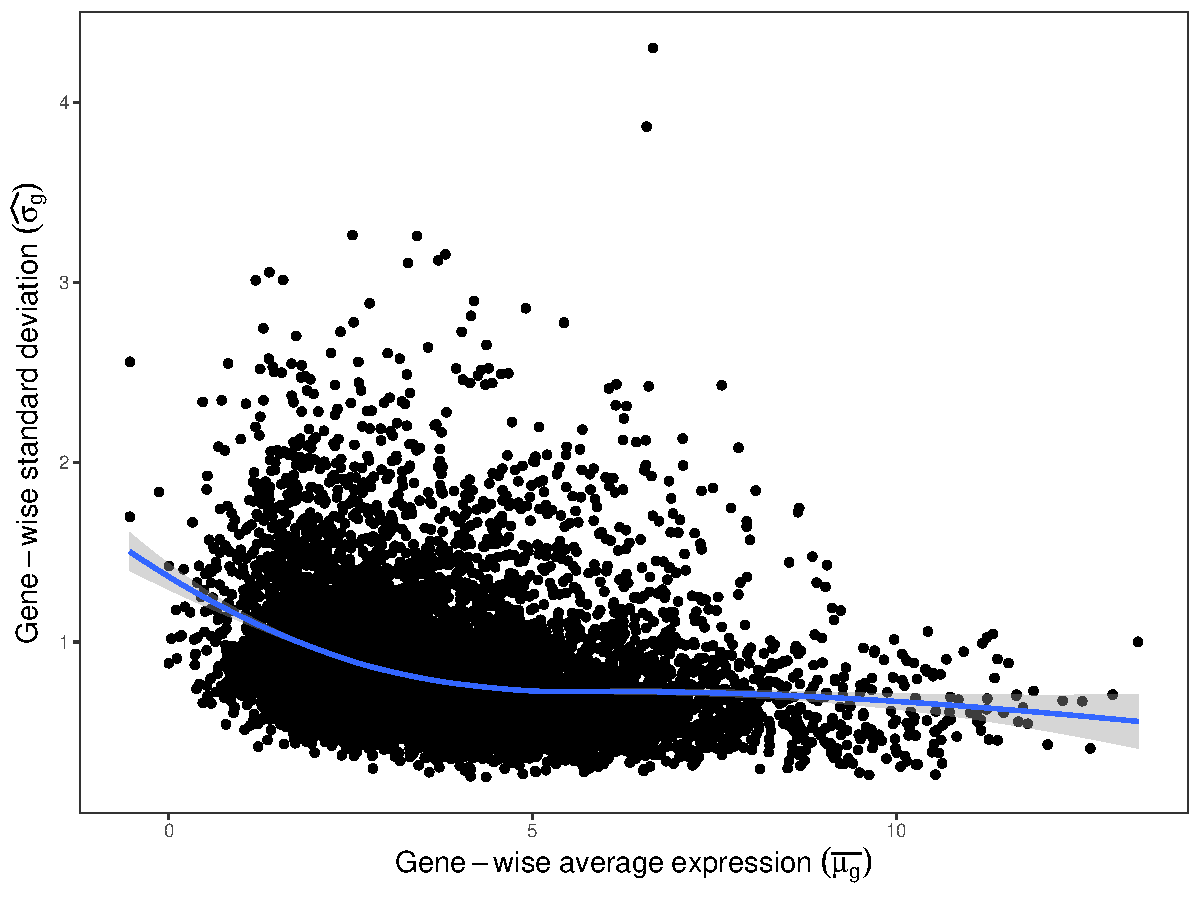
\includegraphics[width=1\linewidth]{sSNAPPY_paper_files/figure-latex/Figure1} 

}

\caption{Schematic illustration of the differences between conventional pathway analysis methods and sSNAPPY. Instead of being limited to treatment-level analyses, \textit{sSNAPPY} allows the detection of pathway perturbation in individual samples by using sample-specific estimates of fold-change instead of experiment-wide estimates. (Created with BioRender.com).}\label{fig:Figure1}
\end{figure}


\begin{figure}

{\centering 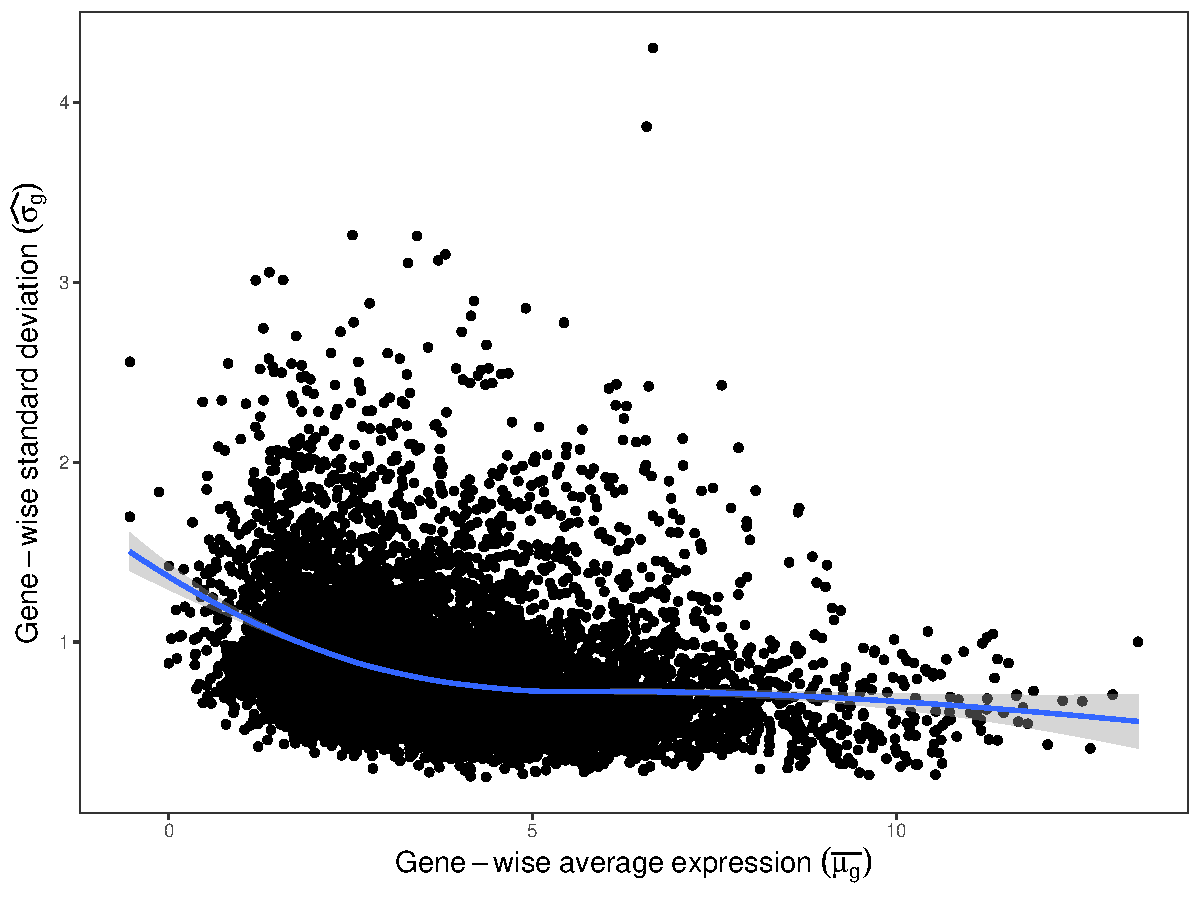
\includegraphics[width=1\linewidth]{sSNAPPY_paper_files/figure-latex/Figure2} 

}

\caption{Gene-wise standard deviations are plotted against the mean logCPM values with mean-variance trend modelled by a loess fit. Whilst standard deviations are shown here for the purposes of visualisation, gene-level weights are calculated using variances at this stage of the sSNAPPY algorithm.}\label{fig:Figure2}
\end{figure}


\begin{figure}

{\centering 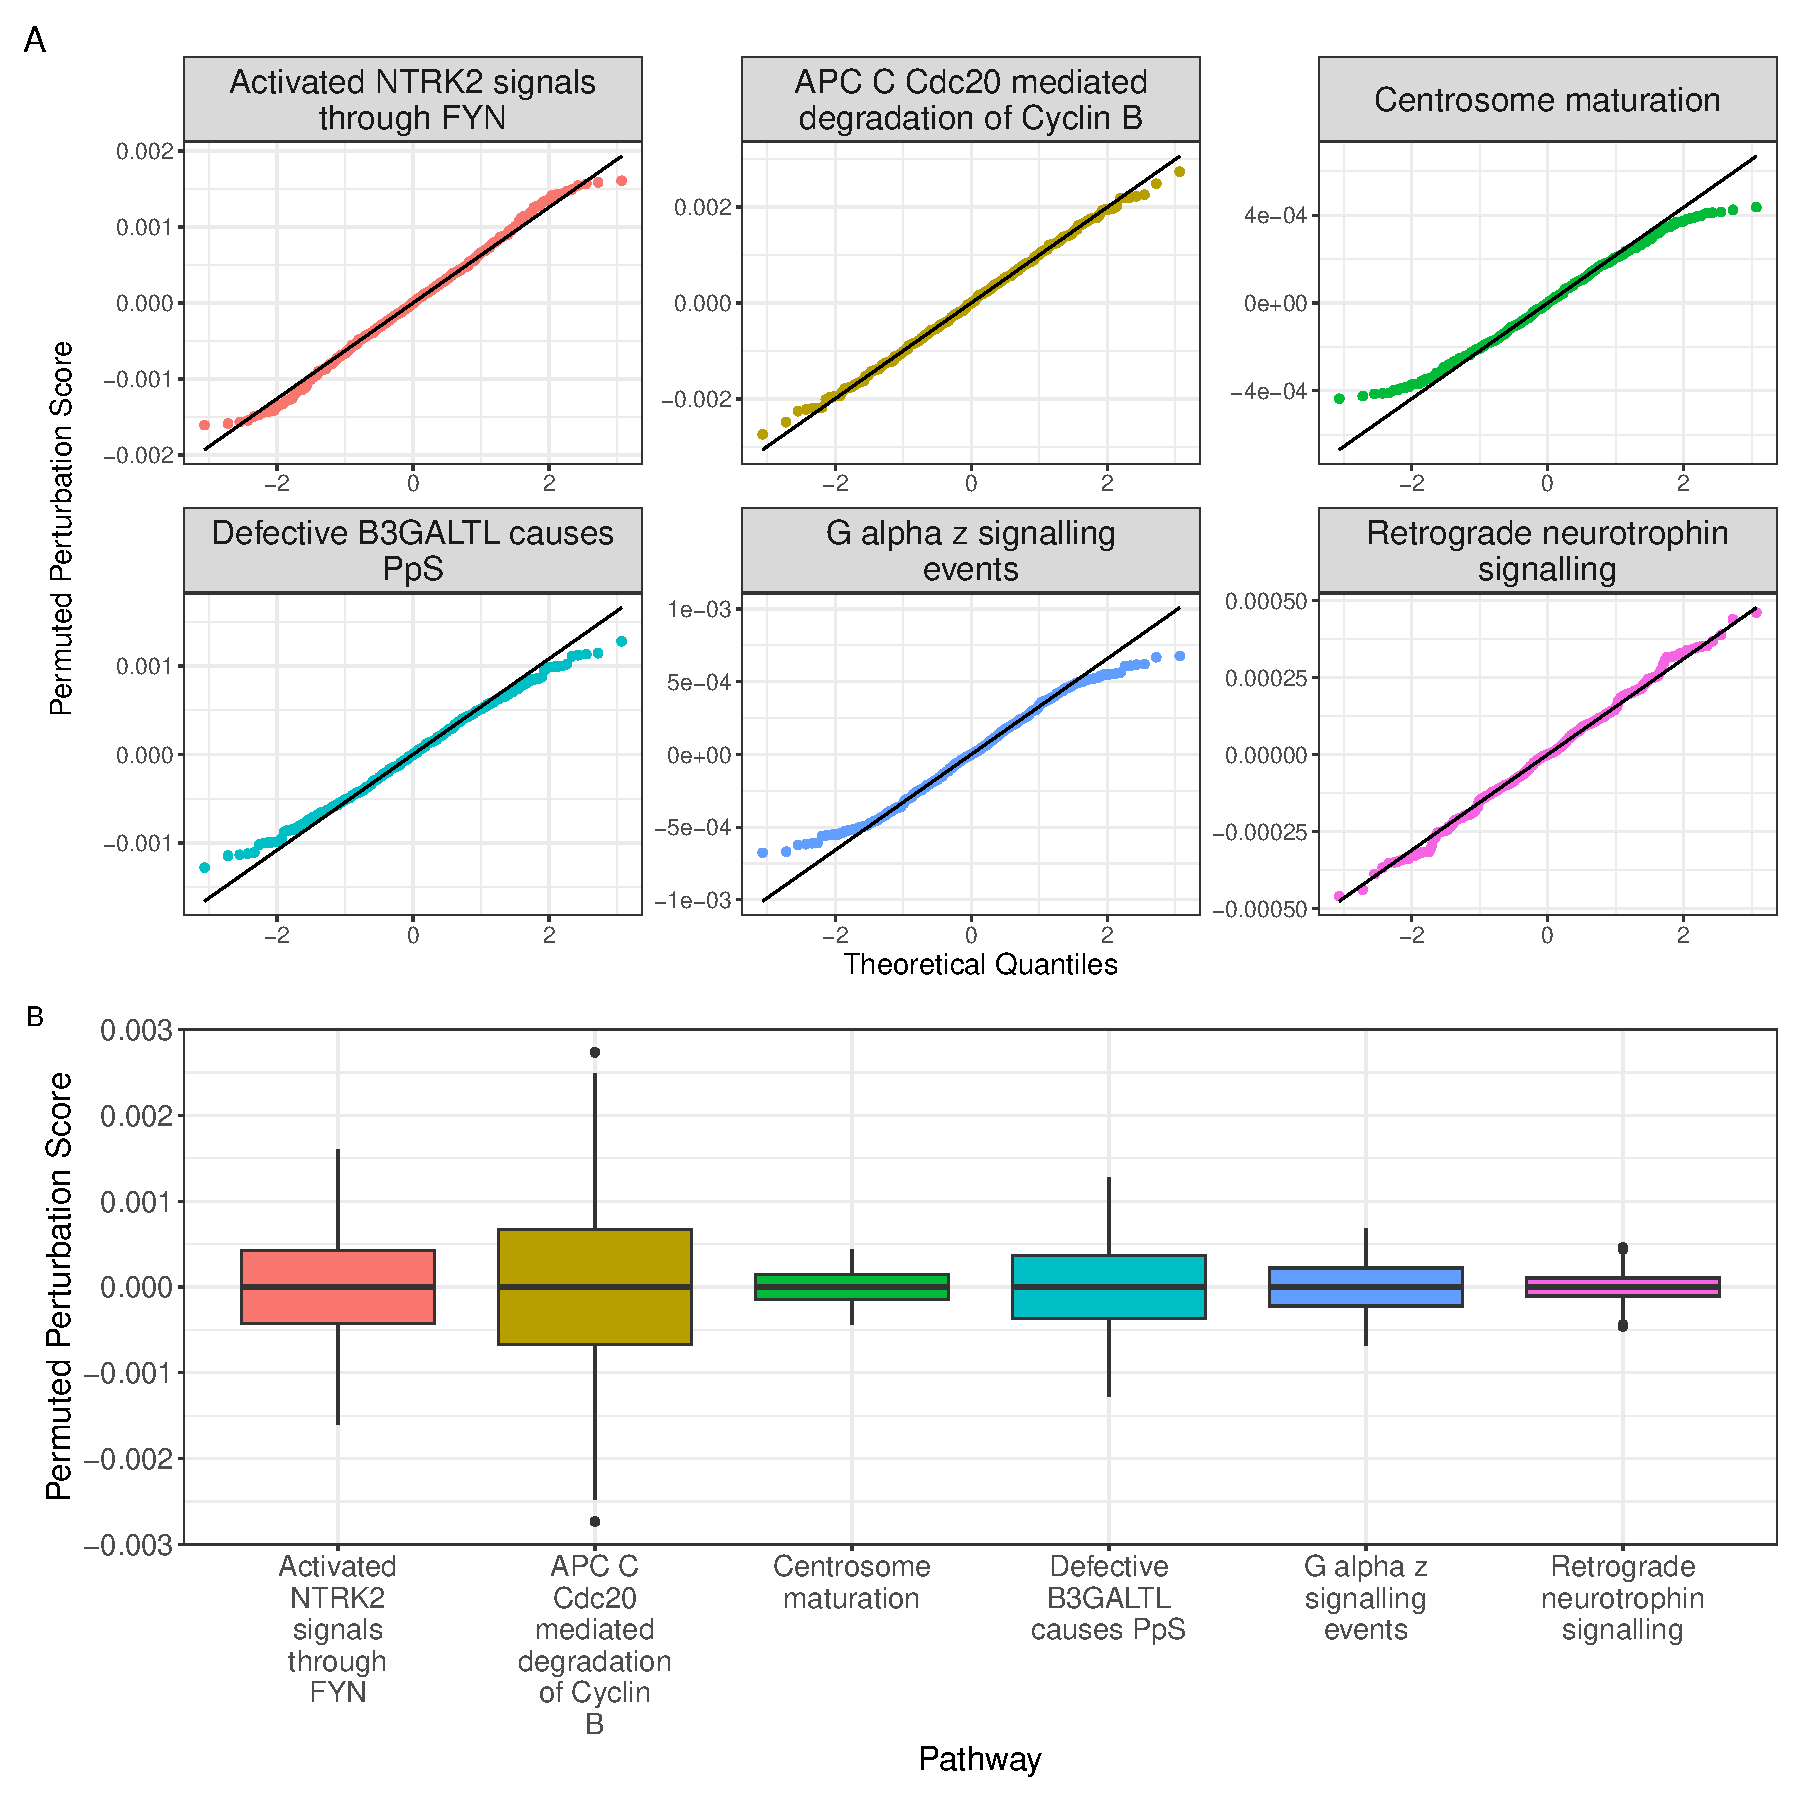
\includegraphics[width=1\linewidth]{sSNAPPY_paper_files/figure-latex/Figure3-1} 

}

\caption{(A) Q-Q plot and (B) distributions of permuted perturbation scores of six randomly selected pathways. All sampled empirical distributions are approximately normally distributed with a mean of zero.}\label{fig:Figure3}
\end{figure}


\begin{figure}

{\centering 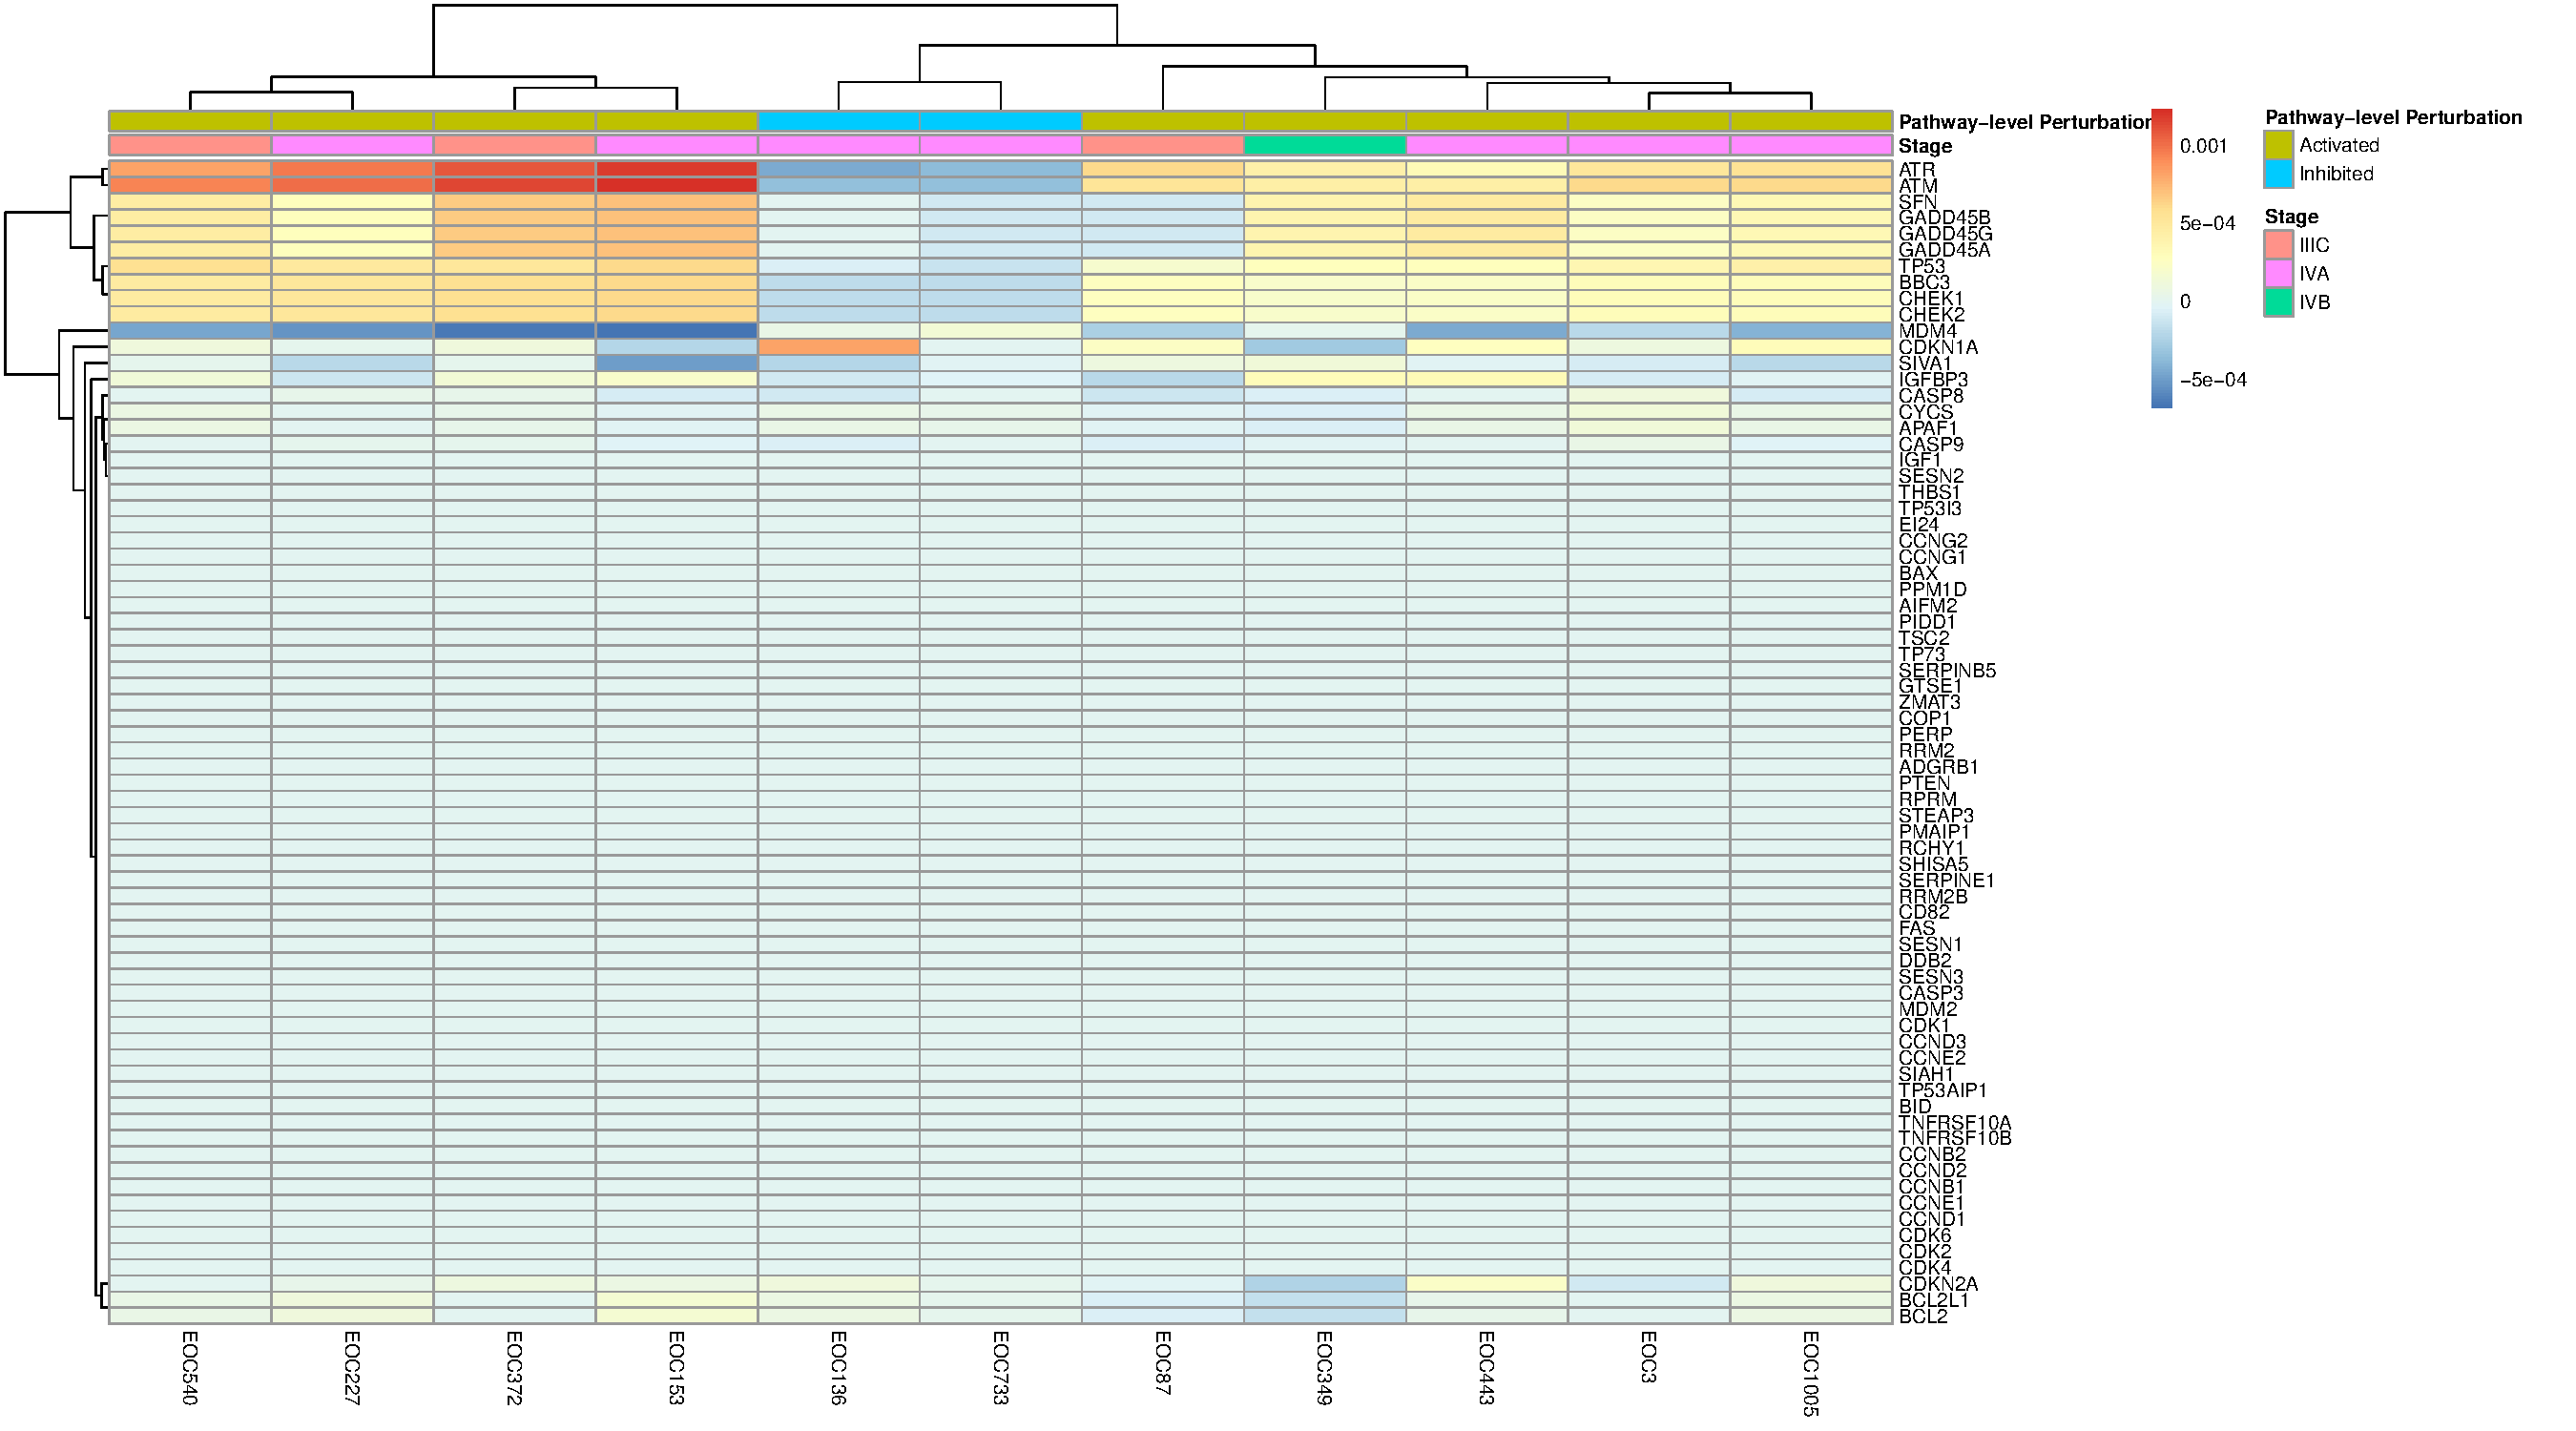
\includegraphics[width=0.9\linewidth]{sSNAPPY_paper_files/figure-latex/Figure4-1} 

}

\caption{Significantly perturbed Reactome pathways identified among post-chemotherapy samples using sSNAPPY, colored by (A) predicted direction of change and (B) -log10(p). Only the 10 most significantly inhibited and 10 most significantly activated pathways are shown.}\label{fig:Figure4}
\end{figure}


\begin{figure}

{\centering 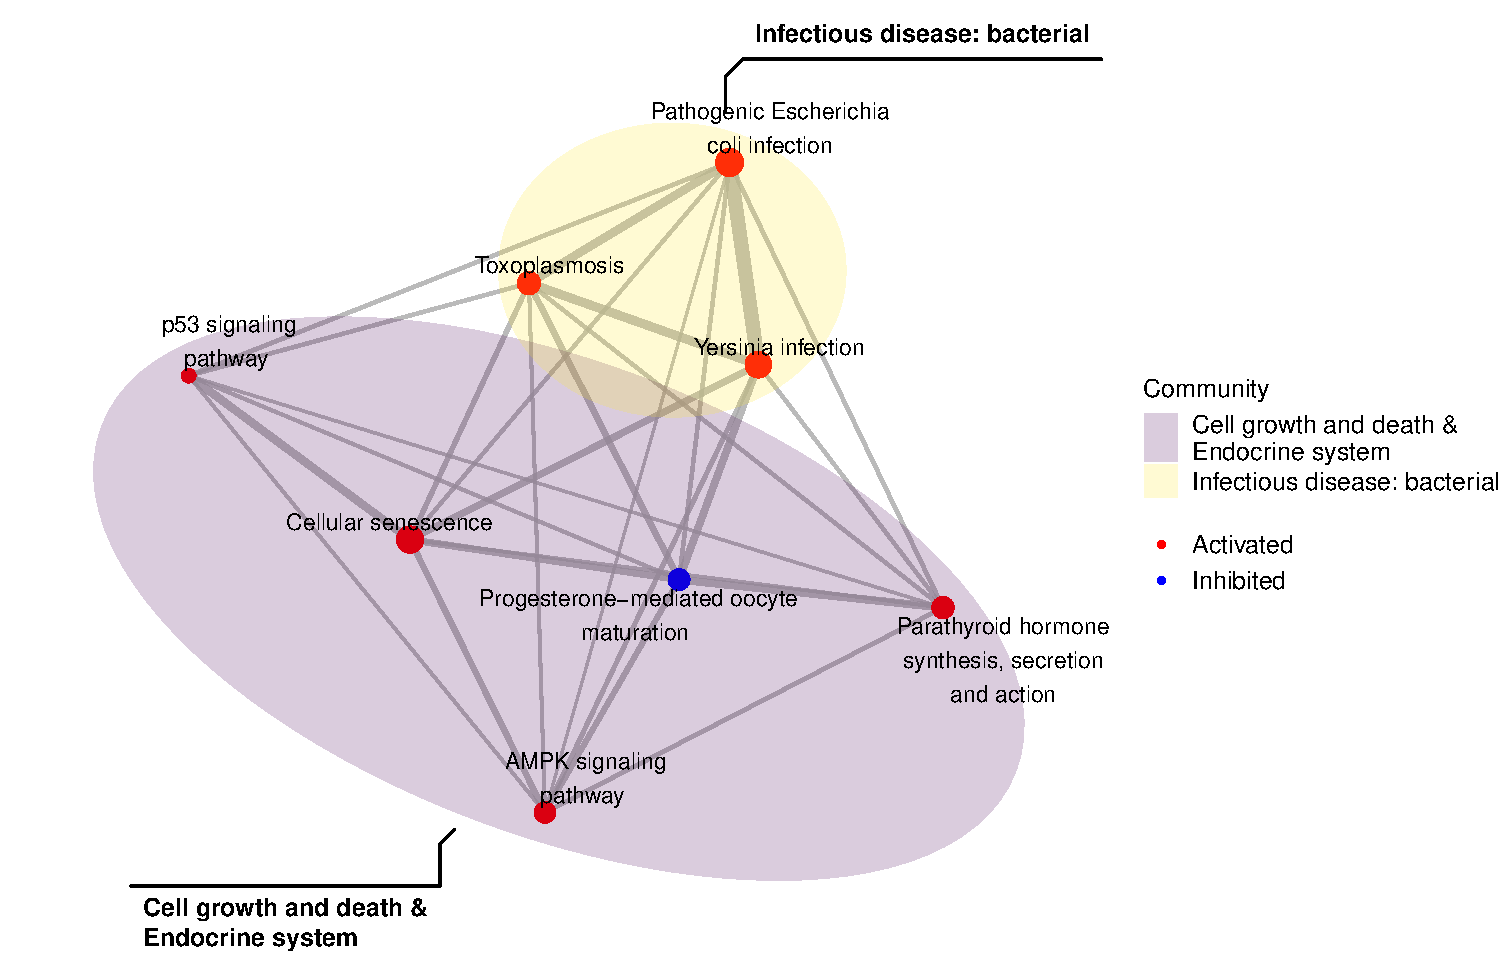
\includegraphics[width=1\linewidth]{sSNAPPY_paper_files/figure-latex/Figure5-1} 

}

\caption{Significantly perturbed Reactome pathways identified among post-chemotherapy samples using sSNAPPY, colored by community structures detected through the louvain algorithm. The main biological processes associated with the top 20 pathways that wer most perturbed by the chemotherapy were shown.}\label{fig:Figure5}
\end{figure}


\begin{figure}

{\centering 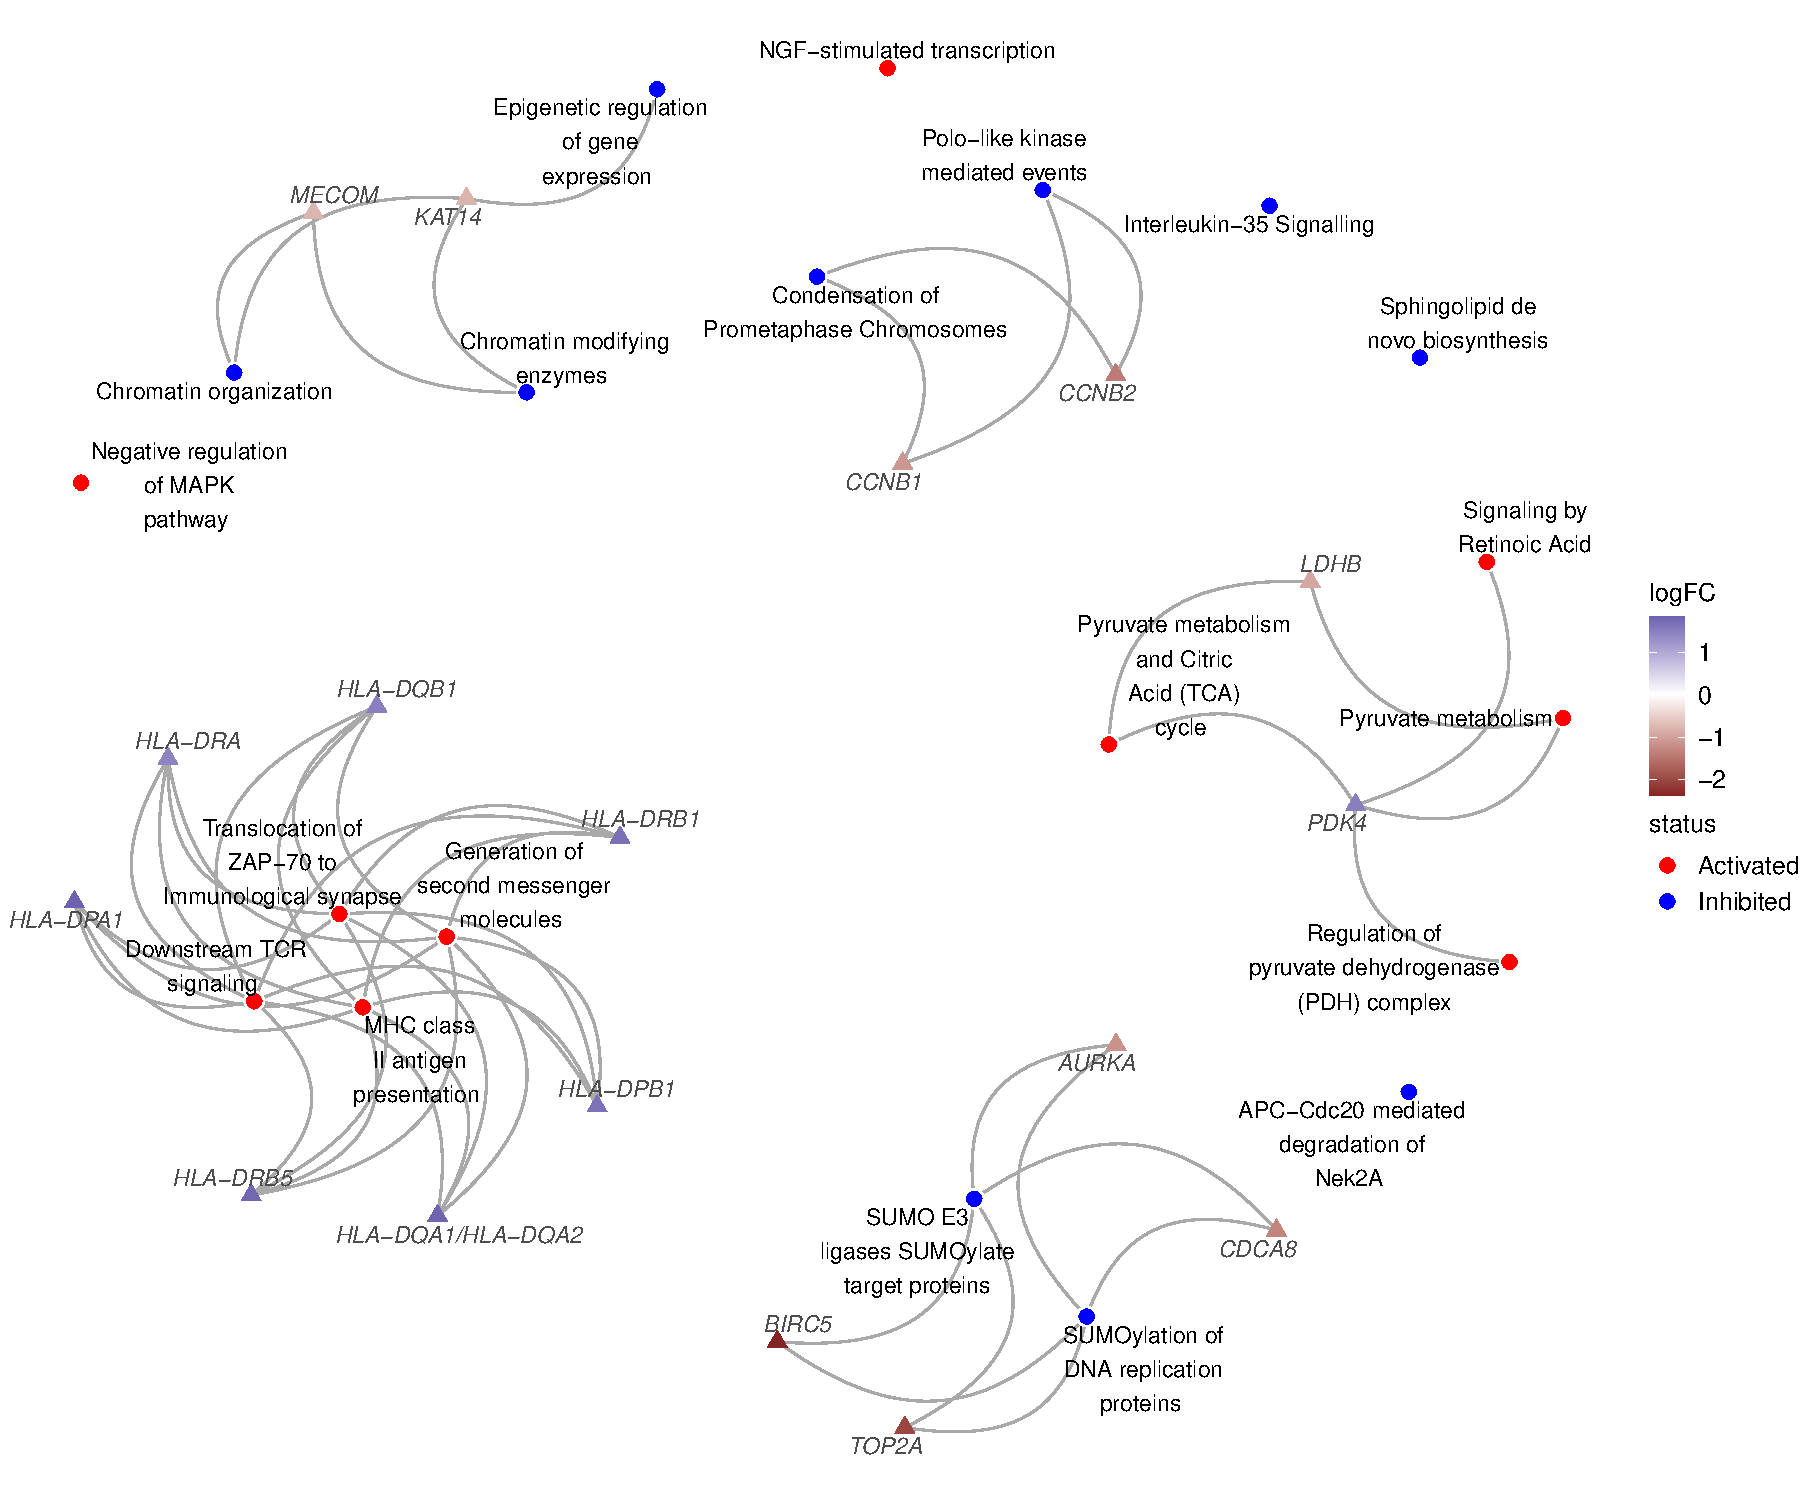
\includegraphics[width=1\linewidth]{sSNAPPY_paper_files/figure-latex/Figure6-1} 

}

\caption{Significantly perturbed Reactome pathways identified among post-chemotherapy samples using sSNAPPY, showing any genes in the top 500 ranked by magnitude of change in expression, and which pathways they are likely contributing to. Only the 10 most significantly inhibited and 10 most significantly activated pathways are shown.}\label{fig:Figure6}
\end{figure}


\begin{figure}

{\centering 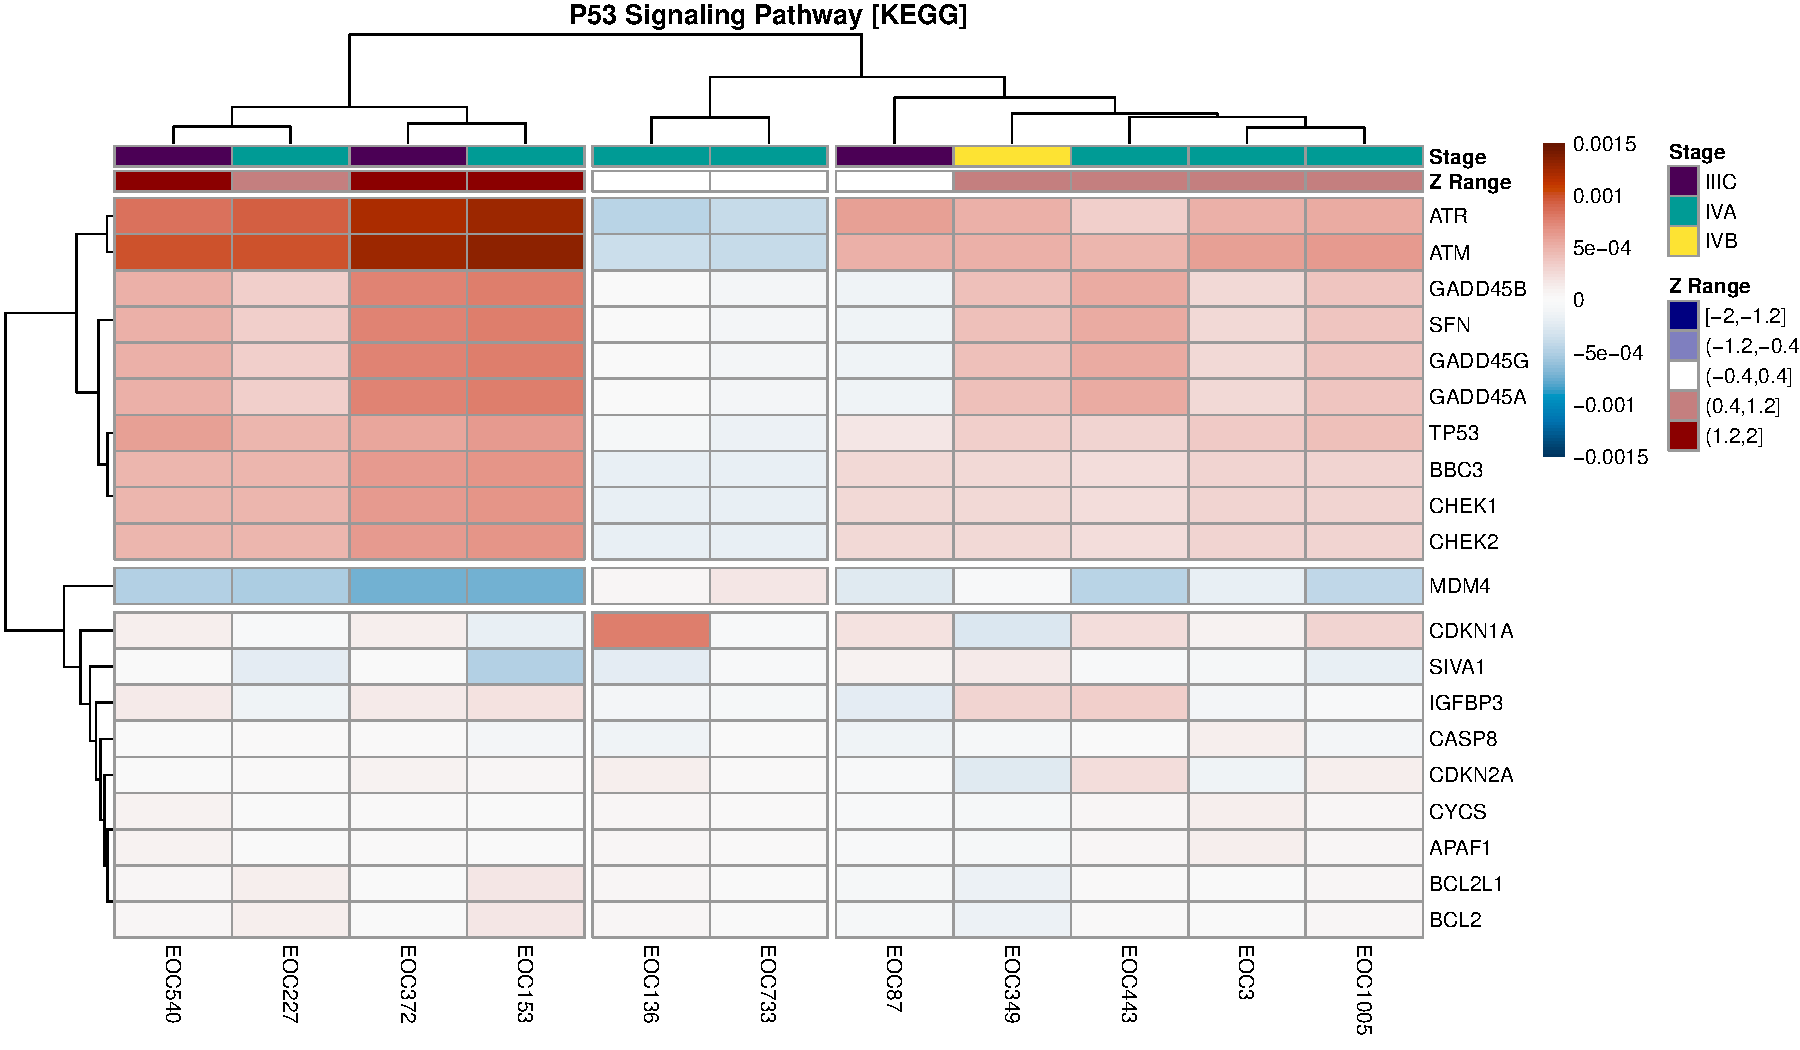
\includegraphics[width=1\linewidth]{sSNAPPY_paper_files/figure-latex/Figure7-1} 

}

\caption{Gene-level perturbation scores for the top 10 genes in the "SUMOylation of DNA replication proteins" pathway ranked by average contribution to the perturbation score. Samples were annotated by patient chemotherapy response score (CRS), along with the range for sample-level Z-scores as a guide to sample-specific pathway perturbation. The genes CDCA8, TOP2A, UBE2I, BIRC5 were identified as possible key drivers of the inhibition of of this pathway.}\label{fig:Figure7}
\end{figure}

\clearpage

\begin{figure}

{\centering 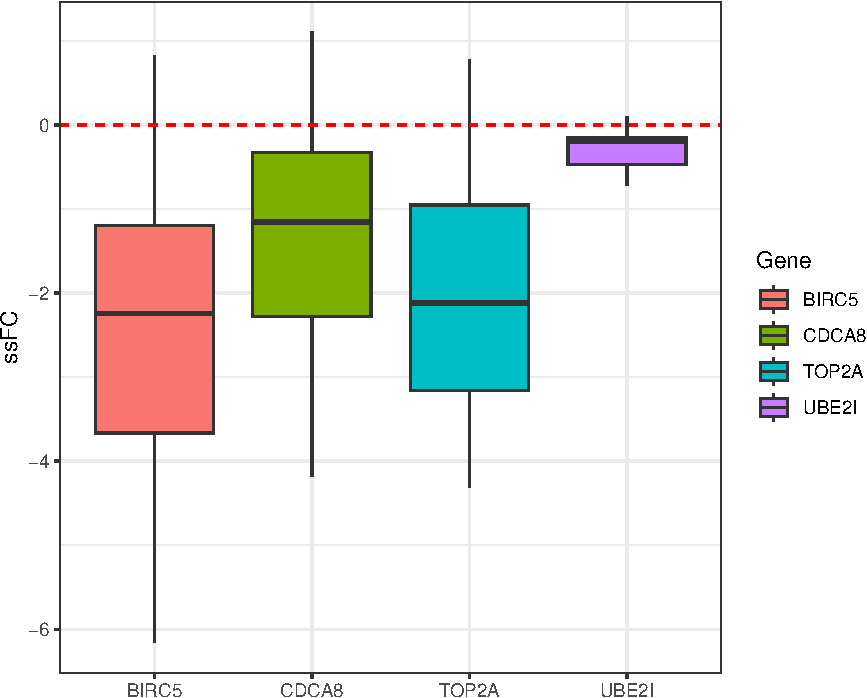
\includegraphics[width=0.8\linewidth]{sSNAPPY_paper_files/figure-latex/Figure8-1} 

}

\caption{Single-sample logFC (ssFC) of potential key genes driving the inhibition of "SUMOylation of DNA replication proteins" pathway as a response to chemotherapy in HGSOC tumours.}\label{fig:Figure8}
\end{figure}


\end{document}
